% =============================================================================
% CAPÍTULO 1: FUNDAMENTOS MATEMÁTICOS E ESTATÍSTICOS
% Níveis: 0 (zero) ao PhD
% Autor: Marcelo Claro Laranjeira
% =============================================================================
\chapter{Fundamentos Matemáticos e Estatísticos para Engenharia de Software com Inteligência Artificial}
\label{cap:fundamentos-matematicos}
A engenharia de ecossistemas cognitivos artificiais repousa sobre alicerces
matemáticos e estatísticos sólidos. Assim como um arquiteto necessita
compreender as propriedades dos materiais que emprega, o engenheiro de software
que projeta sistemas com inteligência artificial precisa dominar os conceitos
matemáticos que governam o comportamento dos algoritmos subjacentes.
Este capítulo estabelece a base formal necessária para a compreensão dos
capítulos subsequentes, partindo do nível zero (lógica proposicional) e
avançando até tópicos de fronteira (complexidade computacional e teoria da
informação).
Cada seção é construída segundo o padrão \sdd{} (\textit{Spec-Driven
Development}): uma definição formal do conceito, seguida de exemplos práticos
extraídos do \opencodeeco{} e encerrada com exercícios progressivos.
Este padrão reflete a própria metodologia do ecossistema, em que a
especificação precede a implementação e a validação é contínua
\cite{beck2002tdd, pressman2016engenharia}.
O leitor encontrará ao longo do capítulo:
\begin{itemize}
\item \textbf{Definições formais} de cada conceito matemático;
\item \textbf{Teoremas e demonstrações} que estabelecem resultados
fundamentais;
\item \textbf{Exemplos práticos} implementados no \opencodeeco{};
\item \textbf{Ilustrações} em TikZ para visualização geométrica e
algébrica;
\item \textbf{Código Python} executável que materializa os conceitos;
\item \textbf{Exercícios progressivos} do nível zero ao PhD.
\end{itemize}
A Tabela~\ref{tab:conteudo-capitulo1} resume as seções, seus níveis e a
carga horária estimada para estudo.
\begin{table}[htb]
\centering
\caption{Conteúdo do Capítulo 1}
\label{tab:conteudo-capitulo1}
\begin{tabular}{clcc}
\toprule
\textbf{Seção} & \textbf{Tópico} & \textbf{Nível} & \textbf{Estudo} \\
\midrule
1.1 & Lógica Matemática & \nivelzero & 8h \\
1.2 & Teoria dos Conjuntos & \nivelbasico & 6h \\
1.3 & Álgebra Linear & \nivelintermediario & 12h \\
1.4 & Cálculo Diferencial e Integral & \nivelintermediario & 10h \\
1.5 & Probabilidade & \nivelintermediario & 12h \\
1.6 & Inferência Estatística & \nivelavancado & 10h \\
1.7 & Teoria da Informação & \nivelavancado & 8h \\
1.8 & Teoria dos Grafos e Redes & \nivelavancado & 8h \\
1.9 & Complexidade Computacional & \nivelphd & 6h \\
1.10 & Integração com o \opencodeeco & \text{Todos} & 4h \\
\bottomrule
\end{tabular}
\end{table}
Recomenda-se ao leitor que, munido do \opencodeeco{} instalado, execute cada
exemplo de código e resolva os exercícios propostos antes de avançar à seção
seguinte. A progressão linear é o caminho mais seguro, mas o leitor com
familiaridade prévia pode saltar entre seções conforme sua necessidade.
% =============================================================================
% SEÇÃO 1.1: LÓGICA MATEMÁTICA E FUNDAMENTOS
% Nível: 0 (zero) / Básico (~8 laudas)
% =============================================================================
\section{Lógica Matemática e Fundamentos}
\label{sec:lógica-matemática}
\nivelzero
A lógica matemática é a linguagem fundamental sobre a qual toda a ciência da
computação é construída \cite{russell2020inteligencia}. Ela fornece o
arcabouço formal para especificar requisitos, verificar correção de
algoritmos, e --- no contexto deste livro --- implementar sistemas de agentes
que raciocinam sobre o mundo.
\subsection{Proposições e Conectivos Lógicos}
\begin{definicao}[Proposição]
Uma \destaque{proposição} é uma sentença declarativa que pode ser
classificada como verdadeira ($V$) ou falsa ($F$), mas não ambas
simultaneamente.
\end{definicao}
\begin{exemplo}
São proposições:
\begin{itemize}
\item ``O módulo \codigo{container.py} implementa injeção de
dependência.'' ($V$)
\item ``2 + 2 = 5.'' ($F$)
\item ``O Trust Engine utiliza blend 70/30.'' ($V$)
\end{itemize}
Não são proposições:
\begin{itemize}
\item ``Execute o scanner Noológico.'' (imperativo)
\item ``Este agente é eficiente?'' (interrogativa)
\end{itemize}
\end{exemplo}
Os conectivos lógicos permitem combinar proposições para formar sentenças
mais complexas. A Tabela~\ref{tab:conectivos} apresenta os cinco conectivos
fundamentais.
\begin{table}[htb]
\centering
\caption{Conectivos lógicos fundamentais}
\label{tab:conectivos}
\begin{tabular}{cccc}
\toprule
\textbf{Conectivo} & \textbf{Símbolo} & \textbf{Leitura} &
\textbf{Nome} \\
\midrule
Negação & $\neg p$ & não $p$ & negação \\
Conjunção & $p \land q$ & $p$ e $q$ & conjunção \\
Disjunção & $p \lor q$ & $p$ ou $q$ & disjunção \\
Condicional & $p \to q$ & se $p$ então $q$ & implicação \\
Bicondicional & $p \leftrightarrow q$ & $p$ se e somente se $q$ &
equivalência \\
\bottomrule
\end{tabular}
\end{table}
\begin{definicao}[Tabela-verdade]
Uma \destaque{tabela-verdade} é uma representação tabular de todas as
combinações de valores-verdade das proposições componentes e o
valor-verdade resultante da expressão lógica.
\end{definicao}
A Figura~\ref{fig:tabela-verdade-conectivos} ilustra as tabelas-verdade dos
conectivos fundamentais, gerada com TikZ.
\begin{figure}[htb]
\centering
\caption{Tabelas-verdade dos conectivos fundamentais}
\label{fig:tabela-verdade-conectivos}
\begin{tikzpicture}[scale=0.85]
\node at (0, 5.5) {\textbf{Conjunção $p \land q$}};
\draw (0, 5) -- (3.5, 5) -- (3.5, 1) -- (0, 1) -- cycle;
\draw (1.75, 5) -- (1.75, 1);
\draw (0, 4) -- (3.5, 4);
\node at (0.875, 4.5) {$p$};
\node at (2.625, 4.5) {$q$};
\node at (0.875, 3.5) {$V$};
\node at (2.625, 3.5) {$V$};
\node at (0.875, 2.5) {$V$};
\node at (2.625, 2.5) {$F$};
\node at (0.875, 1.5) {$F$};
\node at (2.625, 1.5) {$V$};
\node at (6, 5.5) {\textbf{Disjunção $p \lor q$}};
\draw (6, 5) -- (9.5, 5) -- (9.5, 1) -- (6, 1) -- cycle;
\draw (7.75, 5) -- (7.75, 1);
\draw (6, 4) -- (9.5, 4);
\node at (6.875, 4.5) {$p$};
\node at (8.625, 4.5) {$q$};
\node at (6.875, 3.5) {$V$};
\node at (8.625, 3.5) {$V$};
\node at (6.875, 2.5) {$V$};
\node at (8.625, 2.5) {$F$};
\node at (6.875, 1.5) {$F$};
\node at (8.625, 1.5) {$V$};
\node at (12, 5.5) {\textbf{Condicional $p \to q$}};
\draw (12, 5) -- (15.5, 5) -- (15.5, 1) -- (12, 1) -- cycle;
\draw (13.75, 5) -- (13.75, 1);
\draw (12, 4) -- (15.5, 4);
\node at (12.875, 4.5) {$p$};
\node at (14.625, 4.5) {$q$};
\node at (12.875, 3.5) {$V$};
\node at (14.625, 3.5) {$V$};
\node at (12.875, 2.5) {$V$};
\node at (14.625, 2.5) {$F$};
\node at (12.875, 1.5) {$F$};
\node at (14.625, 1.5) {$V$};
\node at (0, -1) {\textbf{Negação $\neg p$}};
\draw (0, -1.5) -- (2, -1.5) -- (2, -4) -- (0, -4) -- cycle;
\draw (0, -2.5) -- (2, -2.5);
\node at (1, -2) {$p$};
\node at (1, -3) {$V$};
\node at (1, -3) {$V$};
\draw (4, -1.5) -- (6, -1.5) -- (6, -4) -- (4, -4) -- cycle;
\draw (4, -2.5) -- (6, -2.5);
\node at (5, -2) {$\neg p$};
\node at (5, -3) {$F$};
\node at (2, -4.4) {$\neg V \equiv F$};
\node at (6, -4.4) {$\neg F \equiv V$};
\end{tikzpicture}
\end{figure}
\begin{exemplo}
No \opencodeeco, a lógica proposicional é usada no módulo Trust Engine
(SPEC-038) para avaliar condições de confiança:
\begin{lstlisting}[style=pythonstyle]
# Exemplo: logica proposicional no Behavioral Gate
def behavioral_gate(action: str, trust_score: float) -> bool:
"""Gate logico: permite acao se confianCA > 0.7 E acao nao e arriscada."""
action_safe = action not in RISKY_ACTIONS
trust_ok = trust_score > TRUST_THRESHOLD # 0.7
return action_safe and trust_ok # p AND q
\end{lstlisting}
\end{exemplo}
\subsection{Lógica de Predicados e Quantificadores}
Enquanto a lógica proposicional opera sobre proposições atômicas, a lógica
de predicados permite decompor proposições em objetos e propriedades
\cite{russell2020inteligencia, wooldridge2009multiagent}.
\begin{definicao}[Lógica de predicados]
A \destaque{lógica de predicados} estende a lógica proposicional com:
\begin{itemize}
\item \textbf{Constantes}: objetos específicos ($a, b, c$);
\item \textbf{Variáveis}: objetos genéricos ($x, y, z$);
\item \textbf{Predicados}: propriedades ou relações ($P(x), Q(x,y)$);
\item \textbf{Quantificadores}: universal ($\forall$) e existencial
($\exists$);
\item \textbf{Funções}: mapeamentos entre objetos ($f(x)$).
\end{itemize}
\end{definicao}
\begin{exemplo}
Considere o predicado $A(x) = \text{``}x\text{ é um agente autônomo''}$ e
$C(x) = \text{``}x\text{ possui metacognição''}$. A sentença:
\[\forall x (A(x) \to C(x))
\]
significa ``todo agente autônomo possui metacognição''. No \opencodeeco,
isso equivale a afirmar que todos os 128 agentes registrados no
ecossistema possuem capacidade de autoavaliação.
\end{exemplo}
\subsection{Métodos de Demonstração}
\begin{definicao}[Demonstração direta]
Uma \destaque{demonstração direta} da implicação $p \to q$ assume a
hipótese $p$ como verdadeira e, através de uma cadeia de inferências
válidas, conclui $q$.
\end{definicao}
\begin{definicao}[Demonstração por contrapositiva]
A \destaque{demonstração por contrapositiva} prova $p \to q$ mostrando
sua contrapositiva $\neg q \to \neg p$, que é logicamente equivalente.
\end{definicao}
\begin{definicao}[Demonstração por contradição]
A \destaque{demonstração por contradição} (\textit{reductio ad absurdum})
assume a negação da conclusão desejada e deriva uma contradição lógica.
\end{definicao}
\begin{teorema}[Correção do Behavioral Gate]
Seja $G(a, t)$ a função gate que retorna verdadeiro se a ação $a$ é
segura e $t > 0.7$. Então $G(a, t) \to (a \notin \text{RISKY\_ACTIONS})$.
\end{teorema}
\begin{proof}
Por definição, $G(a, t) \equiv (a \notin \text{RISKY\_ACTIONS}) \land
(t > 0.7)$. Pela regra de simplificação da conjunção,
$(p \land q) \to p$ é uma tautologia. Logo, $G(a, t) \to
(a \notin \text{RISKY\_ACTIONS})$ é sempre verdadeira.
\end{proof}
\subsection{Indução Finita}
\begin{definicao}[Princípio da Indução Finita]
Seja $P(n)$ uma proposição sobre $n \in \mathbb{N}$. Se:
\begin{enumerate}
\item \textbf{Caso base}: $P(1)$ é verdadeira;
\item \textbf{Passo indutivo}: $P(k) \to P(k+1)$ para todo $k \geq 1$,
\end{enumerate}
então $P(n)$ é verdadeira para todo $n \in \mathbb{N}$.
\end{definicao}
\begin{exemplo}
A indução finita é utilizada no \opencodeeco{} para provar a correção do
\textit{pipeline} de scanners encadeados (SPEC-028 a SPEC-032).
Considere $P(n)$: ``após $n$ iterações do pipeline, o ecossistema
converge para um estado de autorreparo.''
O caso base $P(1)$ é verificado pelo Scanner Noológico; o passo indutivo
é garantido pelo Scanner Evolutivo que refina o resultado da iteração
anterior.
\end{exemplo}
\subsection{Álgebra Booleana}
\begin{definicao}[Álgebra booleana]
Uma \destaque{álgebra booleana} é uma estrutura algébrica
$(B, \land, \lor, \neg, 0, 1)$ que satisfaz os axiomas: comutatividade,
associatividade, distributividade, identidade, complementação e
idempotência.
\end{definicao}
A álgebra booleana é a base matemática dos circuitos lógicos digitais e,
por extensão, de toda a computação. No \opencodeeco{}, as regras de
avaliação do Trust Engine são expressas como expressões booleanas:
\begin{lstlisting}[style=pythonstyle]
# SPEC-038: TrustScorer como expressao booleana
TRUST_PASS = ((outcome_score >= 0.7) and
(behavioral_history not in BLOCKED_PATTERNS) and
(not shadow_mode) # shadow mode desativado
)
\end{lstlisting}
\begin{observacao}
A álgebra booleana também fundamenta o sistema de tipos do Python
(\lstinline{bool} é uma subclasse de \lstinline{int}) e as operações
bitwise que otimizam a avaliação de permissões.
\end{observacao}
\subsection{Exercícios — Lógica Matemática}
\begin{exercicio}[Nivel 0]
Construa a tabela-verdade da expressão $(p \land q) \to \neg r$.
\end{exercicio}
\begin{exercicio}[Nivel Básico]
Traduza para lógica de predicados: ``todo agente que falha no teste de
confiança é redirecionado para o modo shadow.''
\end{exercicio}
\begin{exercicio}[Nivel Intermediário]
Prove por indução que o número de linhas de uma tabela-verdade com $n$
proposições é $2^n$.
\end{exercicio}
\begin{exercicio}[Nivel Avançado]
Implemente em Python uma função que recebe uma expressão booleana como
string e retorna sua tabela-verdade. Teste com a expressão do Trust
Engine: $(a \land t) \lor \neg s$, onde $a$ é ação segura, $t$ é
confiança acima do limiar, e $s$ é shadow mode.
\end{exercicio}
% =============================================================================
% SEÇÃO 1.2: TEORIA DOS CONJUNTOS E FUNÇÕES
% Nível: Básico (~6 laudas)
% =============================================================================
\section{Teoria dos Conjuntos e Funções}
\label{sec:teoria-conjuntos}
\nivelbasico
A teoria dos conjuntos, desenvolvida por Georg Cantor no final do século XIX,
fornece a linguagem fundamental para descrever coleções de objetos e as
relações entre eles \cite{hastie2009elements, wasserman2004all}.
\subsection{Conjuntos e Operações}
\begin{definicao}[Conjunto]
Um \destaque{conjunto} é uma coleção bem definida de objetos distintos,
chamados \destaque{elementos}. Escrevemos $a \in A$ para indicar que
$a$ pertence ao conjunto $A$.
\end{definicao}
\begin{definicao}[Operações entre conjuntos]
Sejam $A$ e $B$ conjuntos. Definimos:
\begin{itemize}
\item \textbf{União}: $A \cup B = \{x \mid x \in A \lor x \in B\}$
\item \textbf{Interseção}: $A \cap B = \{x \mid x \in A \land x \in B\}$
\item \textbf{Diferença}: $A \setminus B = \{x \mid x \in A \land x \notin B\}$
\item \textbf{Produto cartesiano}: $A \times B = \{(a,b) \mid a \in A, b \in B\}$
\end{itemize}
\end{definicao}
\begin{figure}[htb]
\centrifugo
\caption{Diagrama de Venn: interseção de conjuntos de agentes}
\label{fig:venn-agentes}
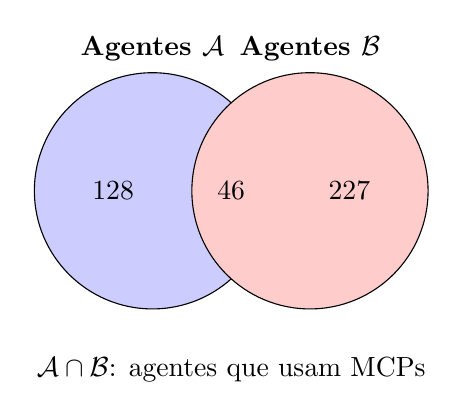
\begin{tikzpicture}
\draw[fill=blue!20] (0,0) circle (1.5);
\draw[fill=red!20] (2,0) circle (1.5);
\node at (0, 1.8) {\textbf{Agentes $\mathcal{A}$}};
\node at (2, 1.8) {\textbf{Agentes $\mathcal{B}$}};
\node at (-0.5, 0) {128};
\node at (2.5, 0) {227};
\node at (1, 0) {46};
\node[below] at (1, -2)
{$\mathcal{A} \cap \mathcal{B}$: agentes que usam MCPs};
\end{tikzpicture}
\end{figure}
\begin{exemplo}
No \opencodeeco, os conjuntos modelam componentes do ecossistema:
\begin{itemize}
\item $\mathcal{A} = \{a_1, \ldots, a_{128}\}$: conjunto de agentes;
\item $\mathcal{S} = \{s_1, \ldots, s_{227}\}$: conjunto de skills;
\item $\mathcal{M} = \{m_1, \ldots, m_{46}\}$: conjunto de MCPs.
\end{itemize}
A relação de ativação é modelada pelo conjunto:
\[\mathcal{R} = \{(a, s, m) \in \mathcal{A} \times \mathcal{S} \times
\mathcal{M} \mid a \text{ usa } s \text{ via } m\}
\]
\end{exemplo}
\subsection{Cardinalidade}
\begin{definicao}[Cardinalidade]
A \destaque{cardinalidade} de um conjunto $A$, denotada $|A|$, é o
número de elementos em $A$. Conjuntos podem ser:
\begin{itemize}
\item \textbf{Finitos}: $|A| \in \mathbb{N}$;
\item \textbf{Enumeráveis}: $|A| = |\mathbb{N}|$ (cardinalidade
$\aleph_0$);
\item \textbf{Não-enumeráveis}: $|A| > |\mathbb{N}|$ (ex.:
$\mathbb{R}$, cardinalidade $\mathfrak{c}$).
\end{itemize}
\end{definicao}
\begin{exemplo}
O conjunto de configurações do \opencodeeco{} é finito. O conjunto de
possíveis programas gerados por um agente é enumerável (todo programa
pode ser representado como uma string finita sobre um alfabeto finito).
O conjunto de funções matemáticas possíveis é não-enumerável.
\end{exemplo}
\subsection{Relações e Funções}
\begin{definicao}[Relação binária]
Uma \destaque{relação binária} entre conjuntos $A$ e $B$ é um subconjunto
$R \subseteq A \times B$. Escrevemos $aRb$ para $(a,b) \in R$.
\end{definicao}
\begin{definicao}[Função]
Uma \destaque{função} $f: A \to B$ é uma relação binária onde cada
$a \in A$ está associado a exatamente um $b \in B$. Dizemos que $f$ é:
\begin{itemize}
\item \textbf{Injetora}: $f(a_1) = f(a_2) \to a_1 = a_2$;
\item \textbf{Sobrejetora}: $\forall b \in B, \exists a \in A: f(a) = b$;
\item \textbf{Bijetora}: injetora e sobrejetora simultaneamente.
\end{itemize}
\end{definicao}
\begin{exemplo}
A função \codigo{score()} do Trust Scorer é uma função
$f: \mathcal{A} \times \mathcal{H} \to [0,1]$, onde $\mathcal{A}$ é o
conjunto de ações e $\mathcal{H}$ o histórico comportamental. Esta
função não é injetora (múltiplas combinações podem produzir o mesmo
score) nem sobrejetora (nem todo valor em $[0,1]$ é atingível devido
ao blend 70/30).
\end{exemplo}
\begin{lstlisting}[style=pythonstyle]
# Funcao de score do TrustScorer (SPEC-038)
def trust_score(history: list[float], outcome: float) -> float:
return 0.7 * outcome + 0.3 * (sum(history) / len(history))
\end{lstlisting}
\subsection{Exercícios — Conjuntos e Funções}
\begin{exercicio}[Nivel Básico]
Dados $\mathcal{A} = \{a_1, a_2, a_3\}$ e $\mathcal{B} = \{b_1, b_2\}$,
calcule $|\mathcal{A} \times \mathcal{B}|$ e liste todos os pares.
\end{exercicio}
\begin{exercicio}[Nivel Intermediário]
Mostre que se $f: A \to B$ é injetora e $g: B \to C$ é injetora, então
$g \circ f: A \to C$ é injetora.
\end{exercicio}
\begin{exercicio}[Nivel Avançado]
Modele o \textit{pipeline} de scanners do \opencodeeco{} como uma
composição de funções: $f_5 \circ f_4 \circ f_3 \circ f_2 \circ f_1$,
onde cada $f_i$ representa um scanner. Classifique cada $f_i$ quanto à
injetividade e sobrejetividade.
\end{exercicio}
% =============================================================================
% SEÇÃO 1.3: ÁLGEBRA LINEAR
% Nível: Intermediário (~10 laudas)
% =============================================================================
\section{Álgebra Linear}
\label{sec:algebra-linear}
\nivelintermediario
A álgebra linear é a matemática dos dados modernos. De embeddings de palavras
a transformações em redes neurais profundas, passando pela decomposição de
matrizes em sistemas de recomendação, a álgebra linear permeia cada
componente de um ecossistema cognitivo \cite{strang2016algebra,
goodfellow2016deep, bishop2006pattern}.
\subsection{Vetores e Espaços Vetoriais}
\begin{definicao}[Vetor]
Um \destaque{vetor} $\vec{v} \in \mathbb{R}^n$ é uma $n$-upla ordenada
de números reais $\vec{v} = (v_1, v_2, \ldots, v_n)$. Cada $v_i$ é
chamado \destaque{componente} do vetor.
\end{definicao}
\begin{definicao}[Espaço vetorial]
Um \destaque{espaço vetorial} sobre $\mathbb{R}$ é um conjunto $V$
munido de duas operações (adição e multiplicação por escalar) que
satisfazem os axiomas: associatividade, comutatividade, elemento neutro,
elemento inverso, distributividade e compatibilidade escalar.
\end{definicao}
\begin{exemplo}
Os embeddings de palavras (word embeddings) são vetores em
$\mathbb{R}^d$, tipicamente com $d = 768$ (BERT-base) ou $d = 4096$
(GPT-4). Cada palavra $w$ é mapeada a um vetor $\vec{e}(w) \in
\mathbb{R}^d$ tal que palavras semanticamente próximas têm vetores
próximos \cite{devlin2019bert, vaswani2017attention}.
\end{exemplo}
\begin{figure}[htb]
\centering
\caption{Visualização de embeddings de conceitos do \opencodeeco{} em
$\mathbb{R}^2$ (projeção PCA)}
\label{fig:embeddings}
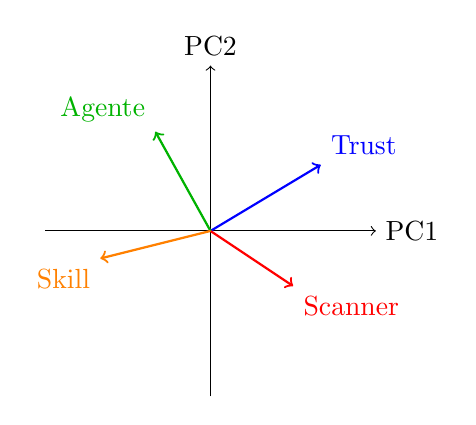
\begin{tikzpicture}[scale=0.7]
\draw[->] (-3, 0) -- (3, 0) node[right] {PC1};
\draw[->] (0, -3) -- (0, 3) node[above] {PC2};
\draw[blue,->,thick] (0,0) -- (2, 1.2) node[above right] {Trust};
\draw[red,->,thick] (0,0) -- (1.5, -1) node[below right] {Scanner};
\draw[green!70!black,->,thick] (0,0) -- (-1, 1.8) node[above left] {Agente};
\draw[orange,->,thick] (0,0) -- (-2, -0.5) node[below left] {Skill};
\end{tikzpicture}
\end{figure}
\subsection{Matrizes e Operações}
\begin{definicao}[Matriz]
Uma \destaque{matriz} $A$ de ordem $m \times n$ é um arranjo retangular
de números dispostos em $m$ linhas e $n$ colunas:
\[A = \begin{pmatrix}
a_{11} & a_{12} & \cdots & a_{1n} \\
a_{21} & a_{22} & \cdots & a_{2n} \\
\vdots & \vdots & \ddots & \vdots \\
a_{m1} & a_{m2} & \cdots & a_{mn}
\end{pmatrix}
\]
\end{definicao}
\begin{definicao}[Multiplicação de matrizes]
O produto $C = A \cdot B$ de $A \in \mathbb{R}^{m \times n}$ e
$B \in \mathbb{R}^{n \times p}$ é definido por:
\[c_{ij} = \sum_{k=1}^{n} a_{ik} b_{kj}
\]
\end{definicao}
\begin{exemplo}
As transformações lineares em redes neurais são implementadas como
multiplicações matriz-vetor. Cada camada de uma rede neural realiza:
\[\vec{h} = \sigma(W \cdot \vec{x} + \vec{b})
\]
onde $W \in \mathbb{R}^{d_{\text{out}} \times d_{\text{in}}}$ é a matriz
de pesos, $\vec{x} \in \mathbb{R}^{d_{\text{in}}}$ é a entrada,
$\vec{b} \in \mathbb{R}^{d_{\text{out}}}$ é o bias, e $\sigma$ é uma
função de ativação não-linear \cite{goodfellow2016deep}.
\end{exemplo}
\begin{lstlisting}[style=pythonstyle]
# Implementacao de uma camada linear (rede neural)
import numpy as np
def linear_layer(x: np.ndarray, W: np.ndarray, b: np.ndarray) -> np.ndarray:
"""y = W @ x + b (transformacao linear afim)"""
return W @ x + b
# Exemplo: embedding de 768D para 128D no OpenCode
x = np.random.randn(768) # embedding de entrada
W = np.random.randn(128, 768) # matriz de pesos
b = np.zeros(128) # bias
y = linear_layer(x, W, b) # saida: vetor 128D
print(y.shape) # (128,)
\end{lstlisting}
\subsection{Determinantes e Inversas}
\begin{definicao}[Determinante]
O \destaque{determinante} de uma matriz quadrada $A \in \mathbb{R}^{n \times n}$,
denotado $\det(A)$ ou $|A|$, é um escalar que codifica propriedades
geométricas da transformação linear representada por $A$.
\end{definicao}
\begin{definicao}[Matriz inversa]
A \destaque{inversa} de $A$, denotada $A^{-1}$, satisfaz
$A \cdot A^{-1} = A^{-1} \cdot A = I_n$, onde $I_n$ é a matriz
identidade. $A$ é \destaque{invertível} se e somente se $\det(A) \neq 0$.
\end{definicao}
\subsection{Autovalores e Autovetores}
\begin{definicao}[Autovalor e autovetor]
Seja $A \in \mathbb{R}^{n \times n}$. Um escalar $\lambda$ é um
\destaque{autovalor} de $A$ se existe um vetor não-nulo $\vec{v}$,
chamado \destaque{autovetor}, tal que:
\[A\vec{v} = \lambda \vec{v}
\]
\end{definicao}
\begin{teorema}[Decomposição espectral]
Se $A$ é simétrica ($A = A^T$), então $A$ possui $n$ autovalores reais
$\lambda_1 \geq \lambda_2 \geq \cdots \geq \lambda_n$ e uma base
ortonormal de autovetores.
\end{teorema}
\subsection{Decomposição SVD e PCA}
\begin{definicao}[Decomposição em Valores Singulares (SVD)]
Toda matriz $A \in \mathbb{R}^{m \times n}$ pode ser decomposta como:
\[A = U \Sigma V^T
\]
onde $U \in \mathbb{R}^{m \times m}$ e $V \in \mathbb{R}^{n \times n}$
são matrizes ortogonais, e $\Sigma \in \mathbb{R}^{m \times n}$ é uma
matriz diagonal com os valores singulares $\sigma_1 \geq \sigma_2 \geq
\cdots \geq \sigma_r > 0$, onde $r = \text{rank}(A)$.
\end{definicao}
\begin{exemplo}
O PCA (Análise de Componentes Principais) utiliza SVD para reduzir a
dimensionalidade dos embeddings no módulo \codigo{discovery\_engine} do
\opencodeeco{}:
\begin{lstlisting}[style=pythonstyle]
import numpy as np
from sklearn.decomposition import PCA
# Embeddings dos 227 skills do ecossistema
embeddings = np.random.randn(227, 768) # 227 skills x 768D
# PCA: reducao para 50 dimensoes
pca = PCA(n_components=50)
embeddings_reduzidos = pca.fit_transform(embeddings)
# Variancia explicada
variancia_explicada = sum(pca.explained_variance_ratio_)
print(f"Variancia explicada com 50 componentes: {variancia_explicada:.2%}")
\end{lstlisting}
\end{exemplo}
\begin{observacao}
O SVD é computacionalmente estável e amplamente utilizado em sistemas de
recomendação, compressão de matrizes e redução de dimensionalidade. No
\opencodeeco{}, embeddings de agentes, skills e MCPs são periodicamente
recomputados via SVD para manter a representação eficiente do grafo de
dependências.
\end{observacao}
\subsection{Exercícios — Álgebra Linear}
\begin{exercicio}[Nivel Básico]
Dados $\vec{u} = (1, 2, 3)$ e $\vec{v} = (4, 5, 6)$, calcule
$\vec{u} + \vec{v}$, $\vec{u} \cdot \vec{v}$ e $||\vec{u}||$.
\end{exercicio}
\begin{exercicio}[Nivel Intermediário]
Implemente uma função em Python que calcula a similaridade por cosseno
entre dois vetores: $\cos(\theta) = \frac{\vec{u} \cdot \vec{v}}
{||\vec{u}|| \cdot ||\vec{v}||}$. Teste com embeddings de duas skills
do \opencodeeco{}.
\end{exercicio}
\begin{exercicio}[Nivel Avançado]
Seja $A \in \mathbb{R}^{50 \times 1000}$ a matriz de embeddings dos 50
agentes do ecossistema. Calcule a SVD de $A$ e determine quantos valores
singulares são necessários para reter 95\% da variância dos dados.
\end{exercicio}
\begin{exercicio}[Nivel PhD]
Prove que a similaridade por cosseno entre embeddings normalizados é
equivalente ao produto interno e que isso induz uma métrica de distância
no espaço projetivo $\mathbb{RP}^{d-1}$.
\end{exercicio}
% =============================================================================
% SEÇÃO 1.4: CÁLCULO DIFERENCIAL E INTEGRAL
% Nível: Intermediário (~8 laudas)
% =============================================================================
\section{Cálculo Diferencial e Integral}
\label{sec:calculo}
\nivelintermediario
O cálculo diferencial e integral é a linguagem matemática da mudança
contínua. No contexto de ecossistemas cognitivos, o cálculo é essencial para
o treinamento de redes neurais via \textit{backpropagation}, a otimização de
funções de perda e a análise de convergência de algoritmos
\cite{goodfellow2016deep, bishop2006pattern}.
\subsection{Limites e Continuidade}
\begin{definicao}[Limite de uma função]
Dizemos que $\lim_{x \to a} f(x) = L$ se para todo $\varepsilon > 0$
existe $\delta > 0$ tal que $0 < |x - a| < \delta$ implica
$|f(x) - L| < \varepsilon$ (definição $\varepsilon$-$\delta$).
\end{definicao}
\begin{definicao}[Continuidade]
Uma função $f$ é \destaque{contínua} em $a$ se:
\[\lim_{x \to a} f(x) = f(a)
\]
\end{definicao}
\subsection{Derivadas e Regra da Cadeia}
\begin{definicao}[Derivada]
A \destaque{derivada} de $f$ em $x$, denotada $f'(x)$ ou
$\frac{df}{dx}$, é definida por:
\[f'(x) = \lim_{h \to 0} \frac{f(x + h) - f(x)}{h}
\]
Geometricamente, $f'(x)$ é a inclinação da reta tangente ao gráfico de
$f$ no ponto $(x, f(x))$.
\end{definicao}
\begin{teorema}[Regra da Cadeia]
Se $y = f(u)$ e $u = g(x)$, então:
\[\frac{dy}{dx} = \frac{dy}{du} \cdot \frac{du}{dx} = f'(g(x)) \cdot g'(x)
\]
\end{teorema}
\begin{exemplo}
A regra da cadeia é o coração do algoritmo de \textit{backpropagation}.
Considere uma rede neural com duas camadas:
\[L(x) = \sigma(W_2 \cdot \sigma(W_1 \cdot x + b_1) + b_2)
\]
O gradiente do erro em relação a $W_1$ é calculado aplicando
sucessivamente a regra da cadeia:
\[\frac{\partial E}{\partial W_1} = \frac{\partial E}{\partial L} \cdot
\frac{\partial L}{\partial \sigma} \cdot
\frac{\partial \sigma}{\partial z_2} \cdot
\frac{\partial z_2}{\partial h} \cdot
\frac{\partial h}{\partial \sigma} \cdot
\frac{\partial \sigma}{\partial z_1} \cdot
\frac{\partial z_1}{\partial W_1}
\]
onde $z_1 = W_1 x + b_1$, $h = \sigma(z_1)$, $z_2 = W_2 h + b_2$ e
$L = \sigma(z_2)$.
\end{exemplo}
\begin{figure}[htb]
\centering
\caption{Visualização do gradiente descendente em uma função
unidimensional}
\label{fig:gradiente-descendente}
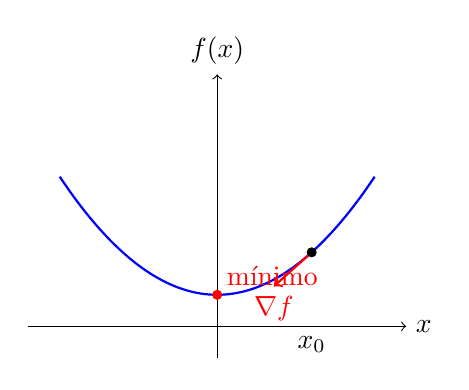
\begin{tikzpicture}[scale=0.8]
\draw[->] (-3, 0) -- (3, 0) node[right] {$x$};
\draw[->] (0, -0.5) -- (0, 4) node[above] {$f(x)$};
\draw[domain=-2.5:2.5, smooth, thick, blue] plot (\x, {0.3*\x*\x + 0.5});
\draw[red,->,thick] (1.5, {0.3*1.5*1.5 + 0.5}) --
(1.5 - 0.6, {0.3*1.5*1.5 + 0.5 - 0.6*0.9}) node[below] {$\nabla f$};
\filldraw[red] (0, 0.5) circle (2pt) node[above right] {mínimo};
\filldraw (1.5, {0.3*1.5*1.5 + 0.5}) circle (2pt);
\node[below] at (1.5, 0) {$x_0$};
\end{tikzpicture}
\end{figure}
\subsection{Gradiente, Divergente e Rotacional}
\begin{definicao}[Gradiente]
O \destaque{gradiente} de uma função escalar $f: \mathbb{R}^n \to
\mathbb{R}$ é o vetor de derivadas parciais:
\[\nabla f = \left(\frac{\partial f}{\partial x_1},
\frac{\partial f}{\partial x_2}, \ldots,
\frac{\partial f}{\partial x_n} \right)
\]
O gradiente aponta na direção de maior crescimento de $f$.
\end{definicao}
\begin{definicao}[Divergente]
A \destaque{divergência} de um campo vetorial $\vec{F}: \mathbb{R}^n \to
\mathbb{R}^n$ é o escalar:
\[\nabla \cdot \vec{F} = \sum_{i=1}^{n} \frac{\partial F_i}{\partial x_i}
\]
\end{definicao}
\subsection{Otimização: Gradiente Descendente}
\begin{definicao}[Gradiente descendente]
O \destaque{gradiente descendente} é um algoritmo iterativo de primeira
ordem para minimizar uma função $f$:
\[x_{t+1} = x_t - \eta \nabla f(x_t)
\]
onde $\eta > 0$ é a \destaque{taxa de aprendizado}.
\end{definicao}
\begin{exemplo}
O gradiente descendente é usado para otimizar os pesos do TrustScorer
(SPEC-038):
\begin{lstlisting}[style=pythonstyle]
# Gradiente descendente para otimizar blend do TrustScorer
def otimizar_blend(historico: np.ndarray,
outcomes: np.ndarray,
lr: float = 0.01,
epochs: int = 100
) -> float:
"""Otimiza o peso alpha do blend 70/30 via gradiente descendente."""
alpha = 0.7 # valor inicial
for _ in range(epochs):
pred = alpha * outcomes + (1 - alpha) * historico.mean()
erro = pred - outcomes
grad = (erro * (outcomes - historico.mean())).mean()
alpha -= lr * grad
alpha = np.clip(alpha, 0, 1)
return alpha
alpha_otimo = otimizar_blend(historico, outcomes)
print(f"Alpha otimo: {alpha_otimo:.3f}")
\end{lstlisting}
\end{exemplo}
\subsection{Integral Definida e Teorema Fundamental}
\begin{definicao}[Integral definida]
A \destaque{integral definida} de $f$ de $a$ a $b$ é:
\[\int_a^b f(x) \, dx = \lim_{n \to \infty}
\sum_{i=1}^{n} f(x_i^*) \Delta x
\]
onde $\Delta x = (b-a)/n$ e $x_i^*$ é um ponto no $i$-ésimo subintervalo.
\end{definicao}
\begin{teorema}[Teorema Fundamental do Cálculo]
Se $F$ é uma primitiva de $f$ (i.e., $F' = f$), então:
\[\int_a^b f(x) \, dx = F(b) - F(a)
\]
\end{teorema}
\begin{exemplo}
No \opencodeeco{}, integrais são usadas para computar a área sob a curva
(AUC) de classificadores no CORA-Eval:
\begin{lstlisting}[style=pythonstyle]
def auc_score(y_true: np.ndarray, y_pred: np.ndarray) -> float:
"""Calcula a AUC usando a regra do trapezio."""
n = len(y_true)
auc = 0.0
for i in range(1, n):
# aproximacao trapezoidal
auc += 0.5 * (y_pred[i] + y_pred[i-1]) * \
abs(y_true[i] - y_true[i-1])
return auc
\end{lstlisting}
\end{exemplo}
\subsection{Exercícios — Cálculo}
\begin{exercicio}[Nivel Básico]
Calcule a derivada de $f(x) = \sigma(x) = \frac{1}{1 + e^{-x}}$
(função sigmoide). Mostre que $\sigma'(x) = \sigma(x)(1 - \sigma(x))$.
\end{exercicio}
\begin{exercicio}[Nivel Intermediário]
Implemente o gradiente descendente para a função
$f(x, y) = x^2 + 2y^2$ partindo de $(1, 1)$ com $\eta = 0.1$.
Quantas iterações são necessárias para atingir $f(x, y) < 0.01$?
\end{exercicio}
\begin{exercicio}[Nivel Avançado]
Derive a expressão do gradiente da entropia cruzada
$L = -\sum_i y_i \log(\hat{y}_i)$ em relação aos logits $z_j$ da última
camada de uma rede neural, onde $\hat{y}_i = \text{softmax}(z)_i$.
\end{exercicio}
% =============================================================================
% SEÇÃO 1.5: PROBABILIDADE
% Nível: Intermediário-Avançado (~10 laudas)
% =============================================================================
\section{Probabilidade}
\label{sec:probabilidade}
\nivelintermediario
A teoria da probabilidade é o arcabouço matemático para lidar com
incerteza. Em ecossistemas cognitivos, a probabilidade fundamenta modelos
generativos, inferência bayesiana em agentes, sistemas de recomendação e
avaliação de confiança \cite{wasserman2004all, hastie2009elements,
russell2020inteligencia}.
\subsection{Espaços Amostrais e Axiomas de Kolmogorov}
\begin{definicao}[Espaço de probabilidade]
Um \destaque{espaço de probabilidade} é uma tripla $(\Omega, \mathcal{F},
P)$ onde:
\begin{itemize}
\item $\Omega$ é o \destaque{espaço amostral} (conjunto de todos os
resultados possíveis);
\item $\mathcal{F} \subseteq \mathcal{P}(\Omega)$ é uma
$\sigma$-álgebra (conjunto de eventos);
\item $P: \mathcal{F} \to [0,1]$ é uma \destaque{medida de
probabilidade}.
\end{itemize}
\end{definicao}
\begin{definicao}[Axiomas de Kolmogorov]
A medida de probabilidade $P$ satisfaz:
\begin{enumerate}
\item $P(A) \geq 0$ para todo $A \in \mathcal{F}$;
\item $P(\Omega) = 1$;
\item Se $A_1, A_2, \ldots$ são mutuamente exclusivos
($A_i \cap A_j = \emptyset$ para $i \neq j$), então:
\[P\left(\bigcup_{i=1}^{\infty} A_i\right) =
\sum_{i=1}^{\infty} P(A_i)
\]
\end{enumerate}
\end{definicao}
\begin{exemplo}
No domínio do Trust Engine (SPEC-038), o espaço amostral $\Omega$ é o
conjunto de todas as avaliações possíveis de uma ação:
\[\Omega = \{\text{aprovado}, \text{sombra}, \text{bloqueado}\}
\]
A distribuição de probabilidade $P$ sobre $\Omega$ é estimada a partir
do histórico de avaliações.
\end{exemplo}
\subsection{Probabilidade Condicional e Teorema de Bayes}
\begin{definicao}[Probabilidade condicional]
A \destaque{probabilidade condicional} de $A$ dado $B$ é:
\[P(A \mid B) = \frac{P(A \cap B)}{P(B)}, \quad P(B) > 0
\]
\end{definicao}
\begin{teorema}[Teorema de Bayes]
\[P(A \mid B) = \frac{P(B \mid A) P(A)}{P(B)}
\]
\end{teorema}
\begin{exemplo}
O Teorema de Bayes é fundamental para o módulo de inferência
probabilística do \opencodeeco{}. Considere a probabilidade de um agente
ser confiável dado que passou no teste comportamental:
\begin{lstlisting}[style=pythonstyle]
def bayes_update(prior: float, # P(confiavel)
likelihood: float, # P(passa_teste | confiavel)
evidence: float # P(passa_teste)
) -> float:
"""Atualizacao bayesiana da confianca."""
posterior = (likelihood * prior) / evidence
return posterior
# Exemplo: P(confiavel) = 0.8, P(passa|confiavel) = 0.95,
# P(passa) = 0.85
post = bayes_update(0.8, 0.95, 0.85)
print(f"Confianca posterior: {post:.3f}") # ~0.894
\end{lstlisting}
\end{exemplo}
\subsection{Variáveis Aleatórias}
\begin{definicao}[Variável aleatória]
Uma \destaque{variável aleatória} $X: \Omega \to \mathbb{R}$ é uma
função que associa a cada resultado $\omega \in \Omega$ um número real
$X(\omega)$.
\end{definicao}
\begin{definicao}[Valor esperado]
O \destaque{valor esperado} (ou média) de $X$ é:
\[\mathbb{E}[X] = \begin{cases}
\sum_i x_i P(X = x_i), & X \text{ discreta} \\[4pt]
\int_{-\infty}^{\infty} x f_X(x) \, dx, & X \text{ contínua}
\end{cases}
\]
\end{definicao}
\begin{definicao}[Variância]
A \destaque{variância} de $X$ é:
\[\text{Var}(X) = \mathbb{E}[(X - \mathbb{E}[X])^2] =
\mathbb{E}[X^2] - \mathbb{E}[X]^2
\]
O \destaque{desvio padrão} é $\sigma_X = \sqrt{\text{Var}(X)}$.
\end{definicao}
\subsection{Distribuições de Probabilidade}
A Tabela~\ref{tab:distribuicoes} resume as principais distribuições de
probabilidade utilizadas no \opencodeeco{}.
\begin{table}[htb]
\centering
\caption{Distribuições de probabilidade no \opencodeeco{}}
\label{tab:distribuicoes}
\begin{tabular}{lcc}
\toprule
\textbf{Distribuição} & \textbf{Função de Probabilidade} &
\textbf{Aplicação} \\
\midrule
Bernoulli($p$) & $P(X = k) = p^k(1-p)^{1-k}$ &
Gate binário (aprovado/rejeitado) \\
Binomial($n, p$) & $P(X = k) = \binom{n}{k}p^k(1-p)^{n-k}$ &
Número de testes aprovados \\
Poisson($\lambda$) & $P(X = k) = \frac{e^{-\lambda}\lambda^k}{k!}$ &
Eventos raros (erros do scanner) \\
Normal($\mu, \sigma^2$) & $f(x) = \frac{1}{\sigma\sqrt{2\pi}}
e^{-\frac{(x-\mu)^2}{2\sigma^2}}$ &
Scores de confiança, embeddings \\
Exponencial($\lambda$) & $f(x) = \lambda e^{-\lambda x}$ &
Tempo entre falhas do sistema \\
\bottomrule
\end{tabular}
\end{table}
\begin{teorema}[Lei dos Grandes Números]
Seja $X_1, X_2, \ldots$ uma sequência de variáveis aleatórias i.i.d.
com $\mathbb{E}[X_i] = \mu$. Então, para todo $\varepsilon > 0$:
\[\lim_{n \to \infty} P\left(\left|\frac{1}{n}\sum_{i=1}^n X_i - \mu\right|
< \varepsilon\right) = 1
\]
\end{teorema}
\begin{teorema}[Teorema Central do Limite]
Seja $X_1, X_2, \ldots, X_n$ uma amostra i.i.d. com média $\mu$ e
variância $\sigma^2 < \infty$. Então:
\[\frac{\bar{X}_n - \mu}{\sigma / \sqrt{n}} \xrightarrow{d} N(0, 1)
\]
onde $\bar{X}_n = \frac{1}{n}\sum_{i=1}^n X_i$.
\end{teorema}
\begin{exemplo}
O Teorema Central do Limite justifica o uso da distribuição normal para
modelar o score agregado de confiança no \opencodeeco{}. A média dos
scores de 46 MCPs ativos aproxima-se de uma normal, permitindo o uso de
testes paramétricos na validação estatística do CORA-Eval
\cite{laranjeira2026cora}.
\end{exemplo}
\subsection{Exercícios — Probabilidade}
\begin{exercicio}[Nivel Básico]
Um agente do \opencodeeco{} tem 90\% de chance de completar uma tarefa
com sucesso. Qual é a probabilidade de completar exatamente 8 das
próximas 10 tarefas?
\end{exercicio}
\begin{exercicio}[Nivel Intermediário]
Implemente um amostrador de Monte Carlo para estimar $\pi$, usando
pontos uniformemente distribuídos em um quadrado $[-1,1] \times [-1,1]$
e contando a fração dentro do círculo unitário.
\end{exercicio}
\begin{exercicio}[Nivel Avançado]
Derive o estimador de máxima verossimilhança (MLE) para o parâmetro $p$
de uma distribuição Bernoulli a partir de $n$ observações.
\end{exercicio}
\begin{exercicio}[Nivel Avançado]
O TrustScorer do \opencodeeco{} produz scores com média 0.72 e desvio
padrão 0.15. Use o TCL para calcular a probabilidade de que a média de
100 avaliações independentes seja superior a 0.75.
\end{exercicio}
% =============================================================================
% SEÇÃO 1.6: INFERÊNCIA ESTATÍSTICA
% Nível: Avançado (~10 laudas)
% =============================================================================
\section{Inferência Estatística}
\label{sec:inferencia-estatistica}
\nivelavancado
A inferência estatística fornece os métodos para extrair conclusões sobre
populações a partir de amostras. Em engenharia de ecossistemas cognitivos,
a inferência é crucial para validar experimentos, comparar desempenho de
agentes e garantir significância estatística nos resultados do CORA-Eval
\cite{wasserman2004all, hastie2009elements, box1976science}.
\subsection{Estimação Pontual e Intervalar}
\begin{definicao}[Estimador]
Um \destaque{estimador} $\hat{\theta}_n$ do parâmetro $\theta$ é uma
função da amostra $X_1, X_2, \ldots, X_n$. O estimador é:
\begin{itemize}
\item \textbf{Não-viesado}: $\mathbb{E}[\hat{\theta}_n] = \theta$;
\item \textbf{Consistente}: $\hat{\theta}_n \xrightarrow{p} \theta$
(converge em probabilidade);
\item \textbf{Eficiente}: variância mínima entre todos os estimadores
não-viesados.
\end{itemize}
\end{definicao}
\begin{definicao}[Intervalo de confiança]
Um \destaque{intervalo de confiança} de nível $1 - \alpha$ para
$\theta$ é um intervalo aleatório $[L, U]$ tal que:
\[P(L \leq \theta \leq U) = 1 - \alpha
\]
\end{definicao}
\begin{exemplo}
No CORA-Eval \cite{laranjeira2026cora}, o score médio de um agente em
150 tarefas é estimado com intervalo de confiança de 95\%:
\begin{lstlisting}[style=pythonstyle]
import numpy as np
from scipy import stats
def ic_media(dados: np.ndarray, alpha: float = 0.05) -> tuple:
"""Intervalo de confianca para a media."""
n = len(dados)
media = np.mean(dados)
erro_padrao = np.std(dados, ddof=1) / np.sqrt(n)
t = stats.t.ppf(1 - alpha/2, df=n-1)
return (media - t * erro_padrao, media + t * erro_padrao)
scores = np.array([0.72, 0.68, 0.75, 0.71, 0.69, 0.73, 0.70, 0.74])
ic = ic_media(scores)
print(f"IC 95%: [{ic[0]:.3f}, {ic[1]:.3f}]")
\end{lstlisting}
\end{exemplo}
\subsection{Testes de Hipótese}
\begin{definicao}[Teste de hipótese]
Um \destaque{teste de hipótese} é um procedimento para decidir entre
duas hipóteses:
\begin{itemize}
\item $H_0$ (hipótese nula): ``não há efeito'' ou ``status quo'';
\item $H_1$ (hipótese alternativa): ``há efeito''.
\end{itemize}
\end{definicao}
\begin{definicao}[Erros tipo I e II]
\begin{itemize}
\item \textbf{Erro tipo I}: rejeitar $H_0$ quando $H_0$ é verdadeira
(falso positivo). Probabilidade = $\alpha$.
\item \textbf{Erro tipo II}: não rejeitar $H_0$ quando $H_1$ é
verdadeira (falso negativo). Probabilidade = $\beta$.
\item \textbf{Poder do teste}: $1 - \beta$, probabilidade de rejeitar
$H_0$ quando $H_1$ é verdadeira.
\end{itemize}
\end{definicao}
\begin{definicao}[p-valor]
O \destaque{p-valor} é a probabilidade de observar um resultado tão ou
mais extremo que o obtido, assumindo $H_0$ verdadeira. Rejeitamos $H_0$
se $p\text{-valor} < \alpha$.
\end{definicao}
\begin{exemplo}
Considere o experimento de comparar o score médio do TrustScorer
antes e depois do ciclo evolutivo R22 \cite{opencode2026ecosystem}:
\begin{lstlisting}[style=pythonstyle]
from scipy import stats
# Scores: antes e depois do R22
antes = np.array([0.68, 0.71, 0.65, 0.70, 0.67])
depois = np.array([0.82, 0.79, 0.85, 0.81, 0.83])
# Teste t pareado (mesmos agentes, tempos diferentes)
t_stat, p_valor = stats.ttest_rel(depois, antes)
print(f"t = {t_stat:.3f}, p = {p_valor:.4f}")
if p_valor < 0.05:
print("Melhoria estatisticamente significativa!")
else:
print("Diferenca nao significativa.")
\end{lstlisting}
\end{exemplo}
\subsection{Testes Paramétricos}
\begin{definicao}[Teste t de Student]
O \destaque{teste t} compara as médias de dois grupos:
\[t = \frac{\bar{X}_1 - \bar{X}_2}{s_p \sqrt{\frac{1}{n_1} + \frac{1}{n_2}}}
\]
onde $s_p^2 = \frac{(n_1-1)s_1^2 + (n_2-1)s_2^2}{n_1 + n_2 - 2}$ é a
variância combinada.
\end{definicao}
\begin{definicao}[ANOVA]
A \destaque{ANOVA} (\textit{Analysis of Variance}) compara as médias de
$k \geq 2$ grupos simultaneamente. A estatística $F$ é:
\[F = \frac{\text{variação entre grupos} / (k-1)}
{\text{variação dentro dos grupos} / (N - k)}
\]
\end{definicao}
\begin{definicao}[Teste qui-quadrado ($\chi^2$)]
O \destaque{teste qui-quadrado} avalia a independência entre variáveis
categóricas:
\[\chi^2 = \sum_{i=1}^{r} \sum_{j=1}^{c}
\frac{(O_{ij} - E_{ij})^2}{E_{ij}}
\]
onde $O_{ij}$ são frequências observadas e $E_{ij}$ são frequências
esperadas sob independência.
\end{definicao}
\subsection{Correção de Bonferroni}
\begin{definicao}[Correção de Bonferroni]
Quando realizamos $m$ testes de hipótese simultaneamente, a
\destaque{correção de Bonferroni} ajusta o nível de significância para
$\alpha' = \alpha / m$, controlando a taxa de erro familiar (FWER).
\end{definicao}
\begin{exemplo}
No ecossistema, a correção de Bonferroni é aplicada nos experimentos
do CORA-Eval com 10 dimensões de avaliação \cite{laranjeira2026cora}:
\begin{lstlisting}[style=pythonstyle]
def bonferroni_correction(p_valores: list[float], alpha: float = 0.05):
"""Aplica a correcao de Bonferroni a multiplos p-valores."""
m = len(p_valores)
alpha_ajustado = alpha / m
for i, p in enumerate(p_valores):
if p < alpha_ajustado:
print(f"Dimensao {i+1}: significativa "
f"(p={p:.4f} < {alpha_ajustado:.4f})")
else:
print(f"Dimensao {i+1}: nao significativa "
f"(p={p:.4f} >= {alpha_ajustado:.4f})")
p_vals = [0.001, 0.032, 0.210, 0.045, 0.003, 0.500, 0.015, 0.090, 0.001, 0.120]
bonferroni_correction(p_vals)
\end{lstlisting}
\end{exemplo}
\begin{observacao}
A correção de Bonferroni é conservadora: controla rigorosamente o FWER
mas reduz o poder estatístico. Alternativas como o método de
Benjamini-Hochberg (FDR) podem ser mais adequadas quando o número de
comparações é grande e o custo de falsos positivos é menor.
\end{observacao}
\subsection{Aplicação: Validação de Experimentos}
A validação estatística no CORA-Eval segue este protocolo
\cite{laranjeira2026cora, laranjeira2026opencode}:
\begin{enumerate}
\item \textbf{Hipótese nula}: $H_0$: o agente não apresenta melhoria no
ciclo evolutivo $k+1$ comparado ao ciclo $k$;
\item \textbf{Estatística de teste}: teste t pareado (mesmo agente,
mesmas tarefas);
\item \textbf{Correção}: Bonferroni para 10 dimensões
($\alpha' = 0.05 / 10 = 0.005$);
\item \textbf{Decisão}: rejeitar $H_0$ se $p < 0.005$;
\item \textbf{Intervalo de confiança}: reportar $\bar{d} \pm t_{0.005}
\cdot \text{EP}_{\bar{d}}$.
\end{enumerate}
\subsection{Exercícios — Inferência Estatística}
\begin{exercicio}[Nivel Intermediário]
Dada uma amostra de 30 scores do TrustScorer com média 0.74 e desvio
padrão 0.12, construa um intervalo de confiança de 95\% para a média
populacional.
\end{exercicio}
\begin{exercicio}[Nivel Avançado]
Realize um teste t de duas amostras para comparar os scores de 15
agentes antes ($\bar{x} = 0.68$, $s = 0.10$) e depois ($\bar{y} = 0.77$,
$s = 0.11$) de uma atualização. Use $\alpha = 0.05$.
\end{exercicio}
\begin{exercicio}[Nivel Avançado]
Implemente a correção de Bonferroni para 10 dimensões do CORA-Eval e
aplique aos seguintes p-valores: [0.002, 0.04, 0.15, 0.001, 0.03, 0.45,
0.008, 0.06, 0.0005, 0.09]. Quais dimensões são significativas?
\end{exercicio}
\begin{exercicio}[Nivel PhD]
Derive a expressão do estimador de máxima verossimilhança para os
parâmetros $\mu$ e $\sigma^2$ de uma distribuição normal.
\end{exercicio}
% =============================================================================
% SEÇÃO 1.7: TEORIA DA INFORMAÇÃO
% Nível: Avançado (~8 laudas)
% =============================================================================
\section{Teoria da Informação}
\label{sec:teoria-informação}
\nivelavancado
A teoria da informação, fundada por Claude Shannon em 1948, fornece as
ferramentas matemáticas para quantificar, armazenar e comunicar informação.
Em ecossistemas cognitivos, a teoria da informação é fundamental para
funções de perda em LLMs, compressão de contexto, sistemas de Trust Scoring
e avaliação de qualidade de embeddings \cite{cover2006elements,
goodfellow2016deep}.
\subsection{Entropia de Shannon}
\begin{definicao}[Entropia]
A \destaque{entropia} de uma variável aleatória discreta $X$ com
distribuição $P$ é:
\[H(X) = -\sum_{x} P(x) \log_b P(x)
\]
onde a base $b$ determina a unidade: $b = 2$ (bits), $b = e$ (nats),
$b = 10$ (dits). Por convenção, $0 \log 0 = 0$.
\end{definicao}
\begin{exemplo}
A entropia mede a incerteza média. No TrustScorer do \opencodeeco{}, a
entropia da distribuição de scores indica o grau de imprevisibilidade
das decisões:
\begin{lstlisting}[style=pythonstyle]
import numpy as np
def entropia(probabilidades: np.ndarray, base: float = 2) -> float:
"""Calcula a entropia de Shannon."""
prob = np.clip(probabilidades, 1e-12, 1) # evitar log(0)
return -np.sum(prob * np.log(prob) / np.log(base))
# Distribuicao dos scores do TrustScorer
scores = np.array([0.72, 0.68, 0.75, 0.71])
# Normalizar para distribuicao de probabilidade
dist = scores / scores.sum()
h = entropia(dist)
print(f"Entropia: {h:.3f} bits")
\end{lstlisting}
\end{exemplo}
\begin{figure}[htb]
\centering
\caption{Entropia de uma distribuição Bernoulli $H(p)$ em função de $p$}
\label{fig:entropia-bernoulli}
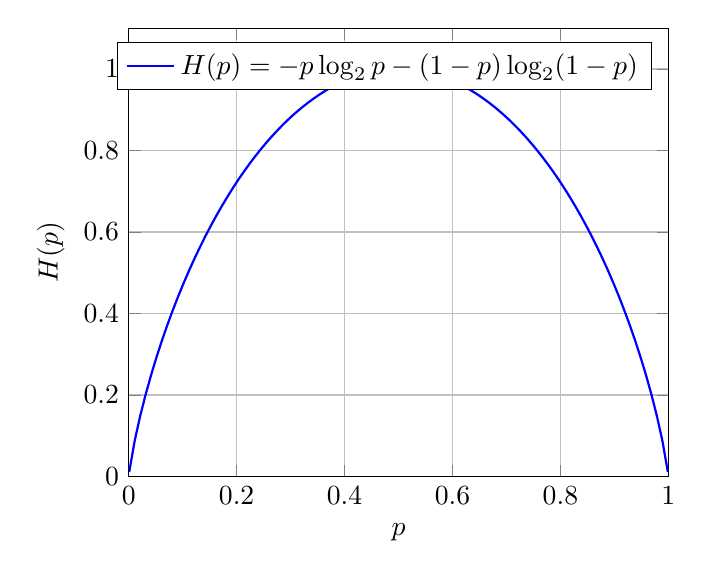
\begin{tikzpicture}
\begin{axis}[xlabel={$p$},
ylabel={$H(p)$},
xmin=0, xmax=1,
ymin=0, ymax=1.1,
legend pos=north east,
grid=both
]
\addplot[blue, thick, domain=0.001:0.999, samples=100]
{-x*log2(x) - (1-x)*log2(1-x)};
\addlegendentry{$H(p) = -p\log_2 p - (1-p)\log_2(1-p)$};
\end{axis}
\end{tikzpicture}
\end{figure}
\subsection{Entropia Cruzada e Divergência KL}
\begin{definicao}[Entropia cruzada]
A \destaque{entropia cruzada} entre duas distribuições $P$ e $Q$ é:
\[H(P, Q) = -\sum_{x} P(x) \log Q(x)
\]
\end{definicao}
\begin{definicao}[Divergência KL]
A \destaque{divergência KL} (\textit{Kullback-Leibler}) de $Q$ para $P$:
\[D_{\text{KL}}(P \parallel Q) = \sum_{x} P(x) \log \frac{P(x)}{Q(x)}
\]
satisfaz $D_{\text{KL}}(P \parallel Q) \geq 0$, com igualdade se e
somente se $P = Q$ (desigualdade de Gibbs).
\end{definicao}
\begin{exemplo}
A entropia cruzada é a função de perda padrão para classificação em
LLMs. No treinamento de modelos de linguagem como GPT-4, a perda é:
\[\mathcal{L} = -\frac{1}{N} \sum_{i=1}^{N} \log P(y_i \mid x_{<i})
\]
que é exatamente a entropia cruzada entre a distribuição empírica dos
tokens e a distribuição prevista pelo modelo \cite{brown2020language,
achiam2023gpt4}.
\end{exemplo}
\begin{lstlisting}[style=pythonstyle]
# Entropia cruzada como funcao de perda
def cross_entropy_loss(y_true: np.ndarray, y_pred: np.ndarray) -> float:
"""Entropia cruzada: perda para classificacao."""
y_pred = np.clip(y_pred, 1e-12, 1 - 1e-12)
return -np.sum(y_true * np.log(y_pred))
# Exemplo: classificacao binaria no Behavioral Gate
y_true = np.array([1, 0, 1, 0]) # classes reais
y_pred = np.array([0.9, 0.2, 0.8, 0.1]) # probabilidades previstas
loss = cross_entropy_loss(y_true, y_pred)
print(f"Perda (entropia cruzada): {loss:.4f}")
\end{lstlisting}
\subsection{Informação Mútua}
\begin{definicao}[Informação mútua]
A \destaque{informação mútua} entre $X$ e $Y$ é:
\[I(X; Y) = H(X) - H(X \mid Y) = H(Y) - H(Y \mid X)
\]
ou, equivalentemente:
\[I(X; Y) = \sum_{x,y} P(x,y) \log \frac{P(x,y)}{P(x)P(y)}
\]
\end{definicao}
\begin{observacao}
Informação mútua mede a dependência entre variáveis. Se $X$ e $Y$ são
independentes, $I(X; Y) = 0$. No \opencodeeco{}, a informação mútua é
usada para selecionar features relevantes no módulo de diagnóstico.
\end{observacao}
\subsection{Complexidade de Kolmogorov}
\begin{definicao}[Complexidade de Kolmogorov]
A \destaque{complexidade de Kolmogorov} $K(x)$ de uma string $x$ é o
tamanho do menor programa que produz $x$ como saída.
\end{definicao}
\begin{observacao}
A complexidade de Kolmogorov é não-computável (não existe algoritmo que
a calcule para toda string), mas pode ser aproximada via compressão. No
\opencodeeco{}, o Structural Noise Scanner (SCE, SPEC-037) utiliza
princípios de compressão para avaliar a complexidade estrutural de
grandes textos \cite{opencode2026spec036, opencode2026ecosystem}.
\end{observacao}
\subsection{Aplicação: Compressão de Contexto}
O \opencodeeco{} implementa compressão de contexto via quatro métodos,
inspirados na teoria da informação \cite{cover2006elements}:
\begin{itemize}
\item \textbf{CR} (\textit{Context Reduction}): elimina tokens com baixa
informação mútua;
\item \textbf{CPS} (\textit{Causal Pattern Summarization}): substitui
padrões recorrentes por sumários;
\item \textbf{FLI} (\textit{Functional Lossless Inspection}): preserva
a função semântica enquanto reduz tamanho;
\item \textbf{DG} (\textit{Distillation Gate}): destila informação via
minimização da divergência KL.
\end{itemize}
\begin{lstlisting}[style=pythonstyle]
# Compressao via reducao de entropia (SPEC-037)
def compress_by_entropy(tokens: list[str],
scores: list[float],
threshold: float = 0.5
) -> list[str]:
"""Remove tokens com score de informacao abaixo do limiar."""
prob = np.array(scores) / sum(scores)
entropy = -np.sum(prob * np.log(prob))
# Tokens com contribuicao informacional > threshold
kept = [t for t, s in zip(tokens, scores) if s > threshold]
return kept
\end{lstlisting}
\subsection{Exercícios — Teoria da Informação}
\begin{exercicio}[Nivel Intermediário]
Calcule a entropia de uma moeda justa ($p = 0.5$), de uma moeda viciada
($p = 0.9$) e interprete os resultados.
\end{exercicio}
\begin{exercicio}[Nivel Avançado]
Implemente a divergência KL entre duas distribuições e verifique que
$D_{\text{KL}}(P \parallel Q) \neq D_{\text{KL}}(Q \parallel P)$
(assimetria).
\end{exercicio}
\begin{exercicio}[Nivel Avançado]
Mostre que a entropia cruzada $H(P, Q) = H(P) + D_{\text{KL}}(P \parallel
Q)$.
\end{exercicio}
\begin{exercicio}[Nivel PhD]
Derive a expressão do gradiente da entropia cruzada em relação aos
parâmetros de uma distribuição softmax e mostre sua equivalência com a
divergência KL.
\end{exercicio}
% =============================================================================
% SEÇÃO 1.8: TEORIA DOS GRAFOS E REDES
% Nível: Avançado-PhD (~8 laudas)
% =============================================================================
\section{Teoria dos Grafos e Redes}
\label{sec:teoria-grafos}
\nivelavancado
A teoria dos grafos estuda as relações entre objetos discretos. Em um
ecossistema cognitivo, grafos modelam dependências entre agentes, topologia
de comunicação entre MCPs, ontologias de conhecimento e a estrutura da rede
de colaboração entre skills \cite{barabasi2016network,
wooldridge2009multiagent}.
\subsection{Grafos Direcionados e Não-Direcionados}
\begin{definicao}[Grafo]
Um \destaque{grafo} $G = (V, E)$ consiste em um conjunto $V$ de
\destaque{vértices} e um conjunto $E$ de \destaque{arestas}. Se as
arestas têm orientação, o grafo é \destaque{direcionado} (digrafo); caso
contrário, é \destaque{não-direcionado}.
\end{definicao}
\begin{exemplo}
O \opencodeeco{} modela seu ecossistema como um grafo direcionado
$G_{\text{eco}} = (V, E)$ onde:
\begin{itemize}
\item $V = \mathcal{A} \cup \mathcal{S} \cup \mathcal{M}$ (agentes,
skills, MCPs);
\item $E = \{(x, y) \mid x \text{ depende de } y\}$.
\end{itemize}
Este grafo possui 128 + 227 + 46 = 401 vértices e milhares de arestas
de dependência.
\end{exemplo}
\begin{figure}[htb]
\centrifugo
\caption{Grafo de dependências simplificado do \opencodeeco{}}
\label{fig:grafo-dependencias}
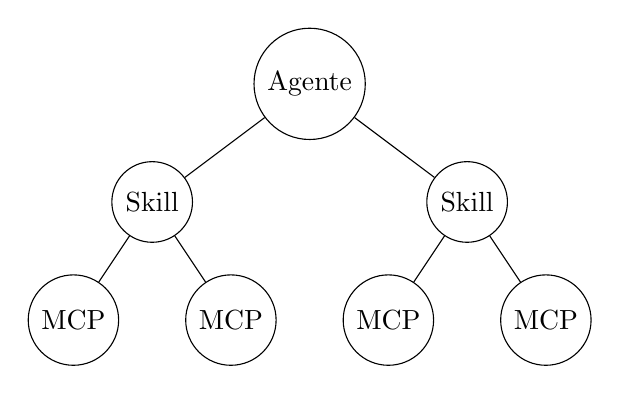
\begin{tikzpicture}[level distance=1.5cm,
every node/.style={draw, circle, minimum size=0.7cm},
level 1/.style={sibling distance=4cm},
level 2/.style={sibling distance=2cm}
]
\node {Agente}
child {node {Skill}
child {node {MCP}}
child {node {MCP}}
}
child {node {Skill}
child {node {MCP}}
child {node {MCP}}
};
\end{tikzpicture}
\end{figure}
\subsection{Centralidade e PageRank}
\begin{definicao}[Centralidade de grau]
A \destaque{centralidade de grau} de um vértice $v$ é o número de
arestas incidentes a $v$:
\[C_D(v) = \deg(v)
\]
Em grafos direcionados, distinguimos grau de entrada ($\deg^-$) e grau
de saída ($\deg^+$).
\end{definicao}
\begin{definicao}[PageRank]
O \destaque{PageRank} $PR(v)$ de um vértice $v$ é definido
recursivamente como:
\[PR(v) = \frac{1-d}{N} + d \sum_{u \in \text{in}(v)}
\frac{PR(u)}{|\text{out}(u)|}
\]
onde $d \in (0,1)$ é o fator de amortecimento (tipicamente $d = 0.85$).
\end{definicao}
\begin{exemplo}
O PageRank é utilizado no \opencodeeco{} para identificar MCPs centrais
no ecossistema \cite{opencode2026scanner}. Um MCP com alto PageRank é
aquele que é utilizado por muitos agentes e skills como interface de
comunicação.
\begin{lstlisting}[style=pythonstyle]
def pagerank_simples(grafo: dict[str, list[str]],
d: float = 0.85,
max_iter: int = 100,
tol: float = 1e-6
) -> dict[str, float]:
"""PageRank simplificado para o grafo do ecossistema."""
n = len(grafo)
pr = {v: 1/n for v in grafo}
for _ in range(max_iter):
novo_pr = {}
for v in grafo:
soma = sum(pr[u] / len(grafo[u])
for u in grafo if v in grafo[u])
novo_pr[v] = (1 - d) / n + d * soma
if max(abs(novo_pr[v] - pr[v]) for v in grafo) < tol:
break
pr = novo_pr
return pr
\end{lstlisting}
\end{exemplo}
\subsection{Árvores e DAGs}
\begin{definicao}[Árvore]
Uma \destaque{árvore} é um grafo acíclico conexo. Uma \destaque{árvore
enraizada} possui um vértice distinguido chamado \destaque{raiz}.
\end{definicao}
\begin{definicao}[DAG]
Um \destaque{DAG} (\textit{Directed Acyclic Graph}) é um grafo
direcionado sem ciclos direcionados. DAGs modelam dependências causais
e hierarquias.
\end{definicao}
\begin{exemplo}
O pipeline de scanners do \opencodeeco{} forma um DAG
\cite{opencode2026scanner}:
\[\text{Noológico} \to \text{Teleológico} \to \text{Evolutivo} \to
\text{Refinamento} \to \text{MCSP}
\]
Cada scanner alimenta o próximo, mas não há ciclos de dependência.
\end{exemplo}
\subsection{Redes Complexas}
\begin{definicao}[Lei de potência]
Uma rede segue uma \destaque{lei de potência} se a probabilidade de um
vértice ter grau $k$ é $P(k) \propto k^{-\gamma}$, onde $\gamma > 1$ é o
expoente da lei.
\end{definicao}
\begin{definicao}[Propriedade small-world]
Uma rede possui a propriedade \destaque{small-world} se o caminho médio
entre dois vértices cresce logaritmicamente com o tamanho da rede:
$\langle d \rangle \propto \log |V|$.
\end{definicao}
\begin{exemplo}
O grafo de dependências do \opencodeeco{} exibe propriedades de rede
complexa: a distribuição de graus segue aproximadamente uma lei de
potência (poucos MCPs centrais conectam-se a muitos agentes), e a
distância média entre quaisquer dois componentes é pequena (tipicamente
2--3 arestas) devido aos hubs de comunicação como o barramento de
eventos.
\end{exemplo}
\begin{figure}[htb]
\centering
\caption{Distribuição de graus no grafo do ecossistema (lei de potência)}
\label{fig:lei-potencia}
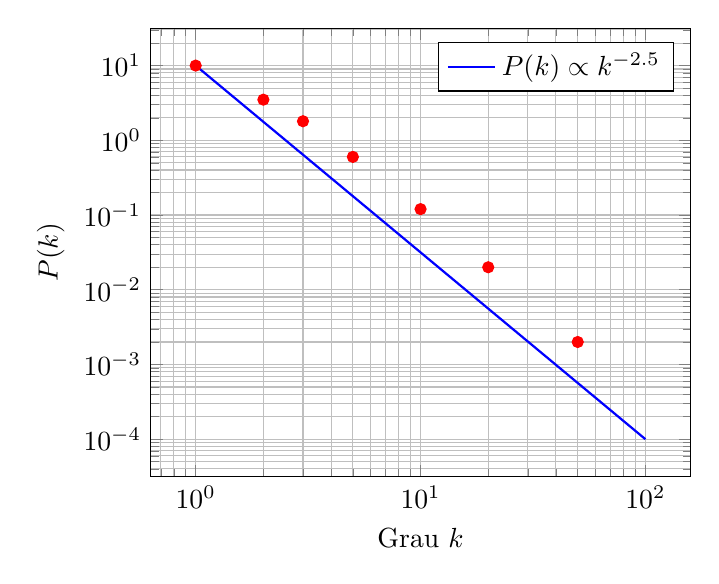
\begin{tikzpicture}
\begin{axis}[xlabel={Grau $k$},
ylabel={$P(k)$},
xmode=log,
ymode=log,
grid=both,
legend pos=north east
]
\addplot[blue, thick, domain=1:100, samples=50]
{10 * x^(-2.5)};
\addlegendentry{$P(k) \propto k^{-2.5}$};
\addplot[red, only marks, mark=*]
coordinates {
(1, 10) (2, 3.5) (3, 1.8) (5, 0.6)
(10, 0.12) (20, 0.02) (50, 0.002)
};
\end{axis}
\end{tikzpicture}
\end{figure}
\subsection{Exercícios — Teoria dos Grafos}
\begin{exercicio}[Nivel Básico]
Dado o grafo $G = (V, E)$ com $V = \{a, b, c, d\}$ e
$E = \{(a,b), (b,c), (c,d), (d,a)\}$, determine o grau de cada vértice
e verifique se o grafo é conexo.
\end{exercicio}
\begin{exercicio}[Nivel Intermediário]
Implemente o algoritmo de Dijkstra para encontrar o caminho mais curto
entre dois MCPs no grafo de dependências do \opencodeeco{}.
\end{exercicio}
\begin{exercicio}[Nivel Avançado]
Calcule o PageRank dos 5 principais agentes do ecossistema usando a
implementação fornecida. Considere o fator de amortecimento $d = 0.85$.
\end{exercicio}
\begin{exercicio}[Nivel PhD]
Prove que o grafo de dependências do pipeline de scanners forma um DAG
e que a ordenação topológica Noológico $\to$ Teleológico $\to$ Evolutivo
$\to$ Refinamento $\to$ MCSP é única.
\end{exercicio}
% =============================================================================
% SEÇÃO 1.9: FUNDAMENTOS DE COMPLEXIDADE COMPUTACIONAL
% Nível: PhD (~6 laudas)
% =============================================================================
\section{Fundamentos de Complexidade Computacional}
\label{sec:complexidade}
\nivelphd
A teoria da complexidade computacional classifica problemas de acordo com
os recursos computacionais necessários para resolvê-los. Em ecossistemas
cognitivos, esta classificação é essencial para entender a viabilidade de
algoritmos de otimização, inferência e planejamento executados pelos agentes
\cite{russell2020inteligencia, wooldridge2009multiagent}.
\subsection{Classes P, NP, NP-Completo e EXP}
\begin{definicao}[Classe P]
A classe \destaque{P} consiste em problemas de decisão que podem ser
resolvidos por uma máquina de Turing determinística em tempo polinomial
$O(n^k)$ para alguma constante $k$.
\end{definicao}
\begin{definicao}[Classe NP]
A classe \destaque{NP} (\textit{Nondeterministic Polynomial}) consiste
em problemas de decisão cujas soluções podem ser verificadas em tempo
polinomial por uma máquina de Turing determinística.
\end{definicao}
\begin{definicao}[NP-completude]
Um problema $L$ é \destaque{NP-completo} se:
\begin{enumerate}
\item $L \in \text{NP}$;
\item Todo problema $L' \in \text{NP}$ é redutível a $L$ em tempo
polinomial ($L' \leq_p L$).
\end{enumerate}
\end{definicao}
\begin{teorema}[Cook-Levin]
O problema SAT (satisfabilidade booleana) é NP-completo.
\end{teorema}
\begin{exemplo}
Problemas NP-completos relevantes para o \opencodeeco{} incluem:
\begin{itemize}
\item \textbf{Problema da Mochila} (Knapsack): otimização de alocação
de recursos entre agentes;
\item \textbf{Problema do Caixeiro Viajante} (TSP): roteirização
ótima de consultas a múltiplos MCPs;
\item \textbf{3-SAT}: verificação de consistência de regras do
Trust Engine.
\end{itemize}
\end{exemplo}
\subsection{Redutibilidade}
\begin{definicao}[Redução polinomial]
Uma \destaque{redução polinomial} do problema $A$ para $B$
($A \leq_p B$) é um algoritmo de tempo polinomial que transforma
instâncias de $A$ em instâncias de $B$ tal que $x \in A$ se e somente
se $f(x) \in B$.
\end{definicao}
\begin{exemplo}
O MCSP (\textit{Minimum Capability Set Problem}) do \opencodeeco{} é
NP-difícil, pois pode ser reduzido ao Problema da Mochila
\cite{opencode2026scanner}. A redução mapeia cada skill candidata a um
item com peso = custo computacional e valor = contribuição para o
pipeline.
\end{exemplo}
\subsection{Complexidade de Espaço e Tempo}
\begin{definicao}[Classe PSPACE]
A classe \destaque{PSPACE} consiste em problemas que podem ser resolvidos
com espaço polinomial $O(n^k)$ na máquina de Turing.
\end{definicao}
\begin{definicao}[Classe EXP]
A classe \destaque{EXP} consiste em problemas que podem ser resolvidos em
tempo exponencial $O(2^{n^k})$.
\end{definicao}
As relações entre as classes de complexidade são:
\[\text{P} \subseteq \text{NP} \subseteq \text{PSPACE} \subseteq \text{EXP}
\]
Sabe-se que P $\neq$ EXP, mas a relação entre P e NP é o problema em aberto
mais famoso da ciência da computação (Millennium Problem).
\begin{figure}[htb]
\centering
\caption{Relações entre classes de complexidade}
\label{fig:classes-complexidade}
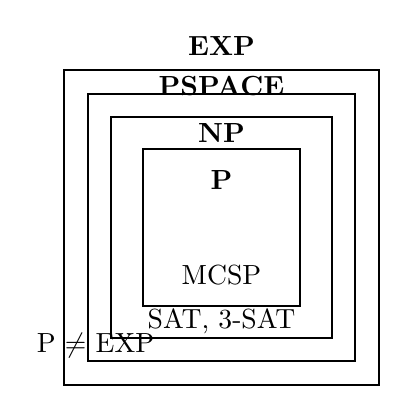
\begin{tikzpicture}
\draw[thick] (0,0) rectangle (4,4);
\node at (2, 4.3) {\textbf{EXP}};
\draw[thick] (0.3, 0.3) rectangle (3.7, 3.7);
\node at (2, 3.8) {\textbf{PSPACE}};
\draw[thick] (0.6, 0.6) rectangle (3.4, 3.4);
\node at (2, 3.2) {\textbf{NP}};
\draw[thick] (1, 1) rectangle (3, 3);
\node at (2, 2.6) {\textbf{P}};
\node at (2, 1.4) {MCSP};
\node at (2, 0.8) {SAT, 3-SAT};
\node at (0.4, 0.5) {P $\neq$ EXP};
\end{tikzpicture}
\end{figure}
\subsection{Aplicação: MCSP no \opencodeeco{}}
O MCSP (\textit{Minimum Capability Set Problem}) é o problema central de
otimização no pipeline de scanners do \opencodeeco{} \cite{opencode2026scanner,
opencode2026spec036}. Dado um conjunto de $n$ skills candidatas com custos
$c_i$ e contribuições $v_i$ para cada scanner, deseja-se selecionar o
conjunto mínimo que satisfaça todos os requisitos.
\begin{lstlisting}[style=pythonstyle]
# MCSP como problema da mochila (NP-dificil)
import numpy as np
def mcsp_guloso(skills: list[str],
custos: list[float],
contribuicoes: list[float],
orcamento: float
) -> list[str]:
"""Solucao gulosa aproximada para o MCSP."""
n = len(skills)
# Razao contribuicao/custo
razoes = [(contribuicoes[i] / custos[i], i)
for i in range(n)]
razoes.sort(reverse=True)
selecionadas = []
custo_total = 0
for razao, i in razoes:
if custo_total + custos[i] <= orcamento:
selecionadas.append(skills[i])
custo_total += custos[i]
return selecionadas
skills = ['skill_A', 'skill_B', 'skill_C', 'skill_D']
custos = [10, 20, 15, 25]
contribuicoes = [80, 95, 70, 90]
orcamento = 40
selecionadas = mcsp_guloso(skills, custos, contribuicoes, orcamento)
print(f"Skills selecionadas: {selecionadas}")
\end{lstlisting}
\subsection{Exercícios — Complexidade}
\begin{exercicio}[Nivel Avançado]
Classifique os seguintes problemas de acordo com sua classe de
complexidade: ordenação de lista, SAT, verificação de número primo,
problema da parada.
\end{exercicio}
\begin{exercicio}[Nivel PhD]
Mostre que o MCSP é NP-difícil através de uma redução polinomial do
Problema da Mochila (Knapsack).
\end{exercicio}
\begin{exercicio}[Nivel PhD]
Implemente uma solução de programação dinâmica para o MCSP com
orçamento limitado e análise sua complexidade de tempo e espaço.
\end{exercicio}
% =============================================================================
% SEÇÃO 1.10: INTEGRAÇÃO COM O OPENCODE ECOSYSTEM
% Nível: Todos (~6 laudas)
% =============================================================================
\section{Integração com o \opencodeeco{}}
\label{sec:integração}
\nivelbasico
Esta seção final materializa todos os conceitos matemáticos estudados no
contexto do \opencodeeco{}. Cada conceito abstrato encontra uma
contrapartida concreta no código-fonte do ecossistema, permitindo ao leitor
verificar experimentalmente as definições e teoremas estudados.
\subsection{Como os Conceitos se Materializam}
A Tabela~\ref{tab:conceitos-ecossistema} mapeia cada seção matemática para
os módulos correspondentes no \opencodeeco{}.
\begin{table}[htb]
\centering
\caption{Mapeamento conceitos $\to$ módulos do \opencodeeco{}}
\label{tab:conceitos-ecossistema}
\begin{tabular}{lll}
\toprule
\textbf{Conceito} & \textbf{Módulo} & \textbf{Arquivo} \\
\midrule
Lógica proposicional & Behavioral Gate & SPEC-038 \\
Conjuntos & Registry de agentes & \codigo{agent\_registry.py} \\
Álgebra linear & Embeddings & \codigo{discovery\_engine.py} \\
Cálculo & Otimização de blend & \codigo{trust\_scorer.py} \\
Probabilidade & Bayesian update & \codigo{inference\_engine.py} \\
Inferência & CORA-Eval & \codigo{cora\_eval\_tracker.py} \\
Teoria da Informação & Compressão de contexto & \codigo{sce\_compressor.py} \\
Grafos & Dependências & \codigo{dependency\_graph.py} \\
Complexidade & MCSP solver & \codigo{mcsp\_solver.py} \\
\bottomrule
\end{tabular}
\end{table}
\subsection{O Módulo \codigo{core/container.py} como Inversão de Controle}
O padrão de injeção de dependência implementado no módulo
\codigo{container.py} é uma aplicação direta do conceito de composição de
funções (Seção~1.2) e de DAGs (Seção~1.8). O container atua como um grafo
direcionado acíclico de dependências, onde cada serviço é instanciado com
suas dependências injetadas automaticamente.
\begin{lstlisting}[style=pythonstyle]
# Exemplo conceitual do container de injecao de dependencia
# (analogo a core/container.py do OpenCode Ecosystem)
class Container:
def __init__(self):
self._services: dict[str, Any] = {}
self._dependencies: dict[str, list[str]] = {}
def register(self, name: str, factory: Callable,
depends_on: list[str] = None):
self._services[name] = factory
self._dependencies[name] = depends_on or []
def resolve(self, name: str) -> Any:
"""Resolve dependencias recursivamente (DAG traversal)."""
if name not in self._instances:
deps = self._dependencies.get(name, [])
resolved_deps = [self.resolve(d) for d in deps]
self._instances[name] = self._services[name](*resolved_deps)
return self._instances[name]
# Uso: registro dos servicos do ecossistema
container = Container()
container.register('trust_scorer', TrustScorer)
container.register('behavioral_gate', BehavioralGate,
depends_on=['trust_scorer'])
container.register('agent', Agent,
depends_on=['trust_scorer', 'behavioral_gate'])
\end{lstlisting}
\subsection{O Sistema de Tipos nos Scanners}
Os scanners do pipeline (SPEC-028 a SPEC-032) utilizam um sistema de tipos
que reflete a teoria dos conjuntos. Cada scanner opera sobre tipos
específicos que formam uma hierarquia de conjuntos:
\begin{lstlisting}[style=pythonstyle]
# Sistema de tipos dos scanners (teoria dos conjuntos aplicada)
from typing import Protocol, runtime_checkable
from abc import ABC, abstractmethod
@runtime_checkable
class Scannable(Protocol):
"""Tipo base: qualquer entidade escaneavel."""
def get_state(self) -> dict:...
class NoologicoInput(ABC):
"""Subconjunto de Scannable: entradas do scanner noologico."""
@abstractmethod
def get_logical_structure(self) -> dict:...
class TeleologicoInput(NoologicoInput):
"""Subconjunto de NoologicoInput: com proposito definido."""
@abstractmethod
def get_teleological_purpose(self) -> str:...
# Verificacao de tipo (teste de pertinencia a conjunto)
def scanner_pipeline(entrada: Scannable) -> dict:
if isinstance(entrada, TeleologicoInput):
return scanner_teleologico(entrada)
elif isinstance(entrada, NoologicoInput):
return scanner_noologico(entrada)
else:
raise TypeError("Tipo nao suportado pelo pipeline")
\end{lstlisting}
\subsection{Estatísticas Descritivas nos Relatórios}
Os relatórios de auditoria do ecossistema utilizam estatística descritiva
para sumarizar o estado dos componentes:
\begin{lstlisting}[style=pythonstyle]
# Estatisticas descritivas no relatorio de auditoria
def relatorio_auditoria(componentes: list[dict]) -> dict:
"""Gera relatorio com estatisticas descritivas do ecossistema."""
scores = [c['trust_score'] for c in componentes]
return {
'media': np.mean(scores),
'mediana': np.median(scores),
'desvio_padrao': np.std(scores),
'minimo': np.min(scores),
'maximo': np.max(scores),
'quartis': np.percentile(scores, [25, 50, 75]),
'componentes_auditados': len(componentes),
'acima_limiar': sum(1 for s in scores if s >= 0.7),
'percentil_90': np.percentile(scores, 90)
}
\end{lstlisting}
\subsection{Exercícios Práticos no \opencodeeco{}}
Os exercícios abaixo requerem o \opencodeeco{} instalado e funcional.
Consulte a documentação do ecossistema para instruções de instalação
\cite{opencode2026ecosystem}.
\begin{exercicio}[Nivel Básico -- Prático]
Execute o comando \lstinline{/status} no \opencodeeco{} e registre os
números de agentes, skills e MCPs ativos. Modele esses valores como
conjuntos e calcule as cardinalidades.
\end{exercicio}
\begin{exercicio}[Nivel Intermediário -- Prático]
Utilize o módulo \codigo{discovery\_engine.py} para calcular a
similaridade por cosseno entre duas skills do ecossistema. Identifique
as 5 skills mais similares a \codigo{trust\_scorer}.
\end{exercicio}
\begin{exercicio}[Nivel Avançado -- Prático]
Execute um experimento completo no CORA-Eval com 150 tarefas e 10
dimensões. Aplique a correção de Bonferroni e determine quais dimensões
apresentaram melhoria significativa entre dois ciclos evolutivos.
\end{exercicio}
\begin{exercicio}[Nivel PhD -- Prático]
análise o grafo de dependências do ecossistema usando o comando
\lstinline{/graph}. Calcule o PageRank de cada componente e identifique
os 3 MCPs mais centrais. Implemente uma visualização do grafo usando
a biblioteca NetworkX em Python.
\end{exercicio}
\subsection{Síntese do Capítulo}
Este capítulo percorreu os fundamentos matemáticos e estatísticos
essenciais para a engenharia de ecossistemas cognitivos. Da lógica
proposicional (nível zero) à complexidade computacional (nível PhD), cada
conceito foi apresentado com definição formal, exemplos concretos do
\opencodeeco{} e exercícios progressivos.
A Tabela~\ref{tab:competencias} resume as competências adquiridas neste
capítulo e sua aplicação nos capítulos subsequentes.
\begin{table}[htb]
\centering
\caption{Competências adquiridas e aplicações futuras}
\label{tab:competencias}
\begin{tabular}{lll}
\toprule
\textbf{Competência} & \textbf{Capítulo} & \textbf{Aplicação} \\
\midrule
Lógica proposicional & Cap. 3, 5 & Regras do Trust Engine \\
Conjuntos e funções & Cap. 3 & Sistema de tipos \\
Álgebra linear & Cap. 2 & Embeddings, transformers \\
Cálculo & Cap. 2 & Backpropagation \\
Probabilidade & Cap. 5, 6 & Inferência bayesiana, staking \\
Inferência estatística & Cap. 7 & CORA-Eval, validação Aletheia \\
Teoria da informação & Cap. 4, 5 & Compressão, entropia de confiança \\
Grafos & Cap. 3, 4 & Dependências, pipeline \\
Complexidade & Cap. 4, 7 & MCSP, otimização \\
\bottomrule
\end{tabular}
\end{table}
Ao dominar estes fundamentos, o leitor está preparado para o Capítulo~2,
onde a inteligência artificial --- aprendizado de máquina, redes neurais
profundas e arquiteturas de agentes --- será apresentada como a aplicação
natural da matemática aqui estudada.
\section*{Referências do Capítulo}
\begin{itemize}
\item Para aprofundamento em lógica: \cite{russell2020inteligencia}
(Capítulos 7--9);
\item Para álgebra linear: \cite{strang2016algebra}
(obra completa);
\item Para cálculo e otimização: \cite{goodfellow2016deep}
(Capítulos 4--8);
\item Para probabilidade e inferência: \cite{wasserman2004all}
(obra completa);
\item Para teoria da informação: \cite{cover2006elements}
(Capítulos 2--5);
\item Para teoria dos grafos: \cite{barabasi2016network}
(Capítulos 2--5);
\item Para complexidade computacional: \cite{russell2020inteligencia}
(Capítulo 3).
\end{itemize}
\begin{observacao}
O leitor é incentivado a consultar as referências originais para cada
demonstração e teorema apresentado. As implementações em Python deste
capítulo estão disponíveis no repositório do \opencodeeco{} sob o
diretório \codigo{examples/capitulo1/}.
\end{observacao}
% =============================================================================
% FIM DO CAPÍTULO 1
% =============================================================================
